\documentclass[12pt,twoside,draft]{book}
\usepackage{../../thesis}
\graphicspath{ {../../images/} }
\usetikzlibrary{arrows,positioning} 
\tikzset{
    %Define standard arrow tip
    >=stealth',
    %Define style for boxes
    box/.style={
           rectangle,
           rounded corners,
           draw=black, very thick,
           text width=6.5em,
           minimum height=2em,
           text centered},
    % Define arrow style
    imply/.style={
           ->,
           thick,
           shorten <=2pt,
           shorten >=2pt},
    both/.style={
           <->,
           thick,
           shorten <=2pt,
           shorten >=2pt,},
    induced/.style={
           dotted,
           ->,
           thick,
           shorten <=2pt,
           shorten >=2pt},
    noimply/.style={
           ->,
           -o,
           thick,
           shorten <=2pt,
           shorten >=50pt}
}

\makeindex
\begin{document}
\chapter{Comparisons of Definitions of Chaos}
We have seen four definitions 
\begin{enumerate}[(i)]
  \item Positive topological entropy
  \item Devaney
  \item Block-Coppel
  \item Li-Yorke
\end{enumerate}
and their variants
\begin{enumerate}[(i)]
  \item Wiggins's (similar to Devaney)
  \item Martelli (equivalent to Wiggins's in $\R^n$)
  \item Marotto (implies Li-Yorke. Requires differentiability)
\end{enumerate}
In this chapter, we discuss the relations between the definitions (i)~(iv).
(Why omit the latter three?)
Throughout this chapter, we consider the dynamical system $(X,F)$, where $X$ is a metric space, and $F$ is a continuous mapping.
More specifically, we consider two cases: a compact interval and compact metric space.
%%%

\section{Compact Interval}
Let $I \subseteq \R$ be a compact interval.
In this section, we consider the case where $X = I$.
As it turns out, Devaney's, Block-Coppel's, and positive topological entropy are equivalent conditions, and any of the three implies Li-Yorke's chaos.
\begin{figure}[ht]
  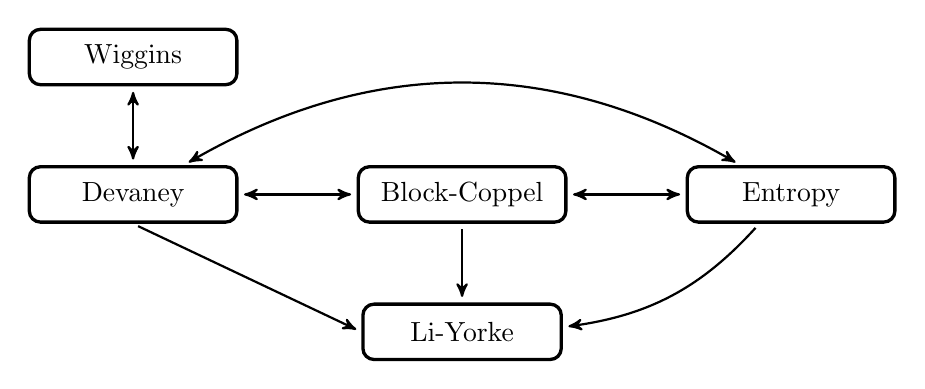
\begin{tikzpicture}[node distance=1cm, auto,]
 %nodes
    \node[box] (ly) {Li-Yorke};
    \node[box, inner sep=5pt,above=1.0cm of ly] (bc) {Block-Coppel};
    \node[box, inner sep=5pt,left=1.5cm of bc] (dev) {Devaney};
    \node[box, inner sep=5pt,right=1.5cm of bc] (ent) {Entropy};
    \node[box, inner sep=5pt,above=1.0cm of dev] (wig) {Wiggins};
 %edges
    \draw[imply] (dev.south) to node[bend right=20] {} (ly.west);  %this guy doesn't bend
    \draw[imply] (ent) to[bend left=20] node {} (ly); 
    \draw[imply] (bc) to node {} (ly); 
    \draw[both] (dev) to[bend left=30] node {} (ent); 
    \draw[both] (dev) to node {} (bc); 
    \draw[both] (dev) to node {} (wig); 
    \draw[both] (bc) to node {} (ent); 
  \end{tikzpicture}
  \label{fig:chaos-interval}
  \caption{
    Relations between the four definitions for a compact interval.
    The three definitions in the first row are all equivalent.
    Li-Yorke's definition is strictly weaker than the other three.
  }
\end{figure}

Devaney's and Block-Coppel's definitions are equivalent.
We already mentioned in the chapter on Devaney's chaos that dense periodic points and topological transitivity imply sensitive dependence on initial conditions in a compact metric space.
Moreover, on a compact interval, topological transitivity implies the existence of dense periodic points.
Thus, Devaney's and Wiggins's definitions are equivalent.
\begin{theorem}
  $(I,F)$ is chaotic in the sense of Devaney if and only if it is chaotic in the sense of Wiggins.
  \label{thm:devaney-wiggins}
  \begin{proof}
    See \citet{silverman}.
  \end{proof}
\end{theorem}
Using the above result, we prove that Devaney's definition is equivalent to Block-Coppel's definition. 
\begin{theorem}
  \citep{aulbach}
  $(I,F)$ is chaotic in Devaney's sense if and only if it is chaotic in Block-Coppel's sense.
  \begin{proof}
    \citep{aulbach}
    (Use \citep{blockcoppel} VI: Proposition 6.)
  \end{proof}
  \label{thm:devaney-blockcoppel}
\end{theorem}

Furthermore, Block-Coppel's definition is equivalent to a mapping having positive topological entropy.
\begin{theorem}
  $(I,F)$ is chaotic in the sense of Block-Coppel if and only if it has positive topological entropy.
  \label{thm:entropy-blockcoppel}
  \begin{proof}
    This follows from Theorem~\ref{thm:devaney-blockcoppel} and Theorem~\ref{thm:devaney-entropy}.
    It is also proved in \citet[VII, Theorem 24]{blockcoppel}.
  \end{proof}
\end{theorem}
Hence, the three definitions---Devaney, Block-Coppel, and positive topological entropy---are equivalent.
Next, we show that Block-Coppel's definition implies Li-Yorke's definition.
\begin{theorem}
  \citep{blockcoppel}
  If $(I,F)$ is chaotic in Block-Coppel's sense, then it is chaotic in Li-Yorke's sense.
  \label{thm:devaney-liyorke}
  \begin{proof}
    See \citet{blockcoppel} (VI; Proposition 27).
  \end{proof}
\end{theorem}
The next example shows that the converse of the previous statement is not true in general.
\begin{example}
  \citep{blockcoppel}
  \label{eg:counterexample}
\end{example}

In summary, Devaney's, Block-Coppel's, and positive topological entropy definitions are equivalent on a compact interval.
Each of the three equivalent definitions imply chaos in Li-Yorke's sense, but Li-Yorke's definition does not imply others.
These results can be proved through other means.
\citet{smital} showed that there exists a Li-Yorke chaotic map that has zero topological entropy.
Also, \citet{omegachaos} showed that Devaney's definition holds if and only if positive topological entropy and vice versa .
%%%

\section{Compact Metric Space}
The result in this more general case is more interesting than the compact interval case.
AKM, Li-Yorke, and Block-Coppel are no longer equivalent to each other.
Moreover, neither of them implies the others.
\begin{figure}[ht]
  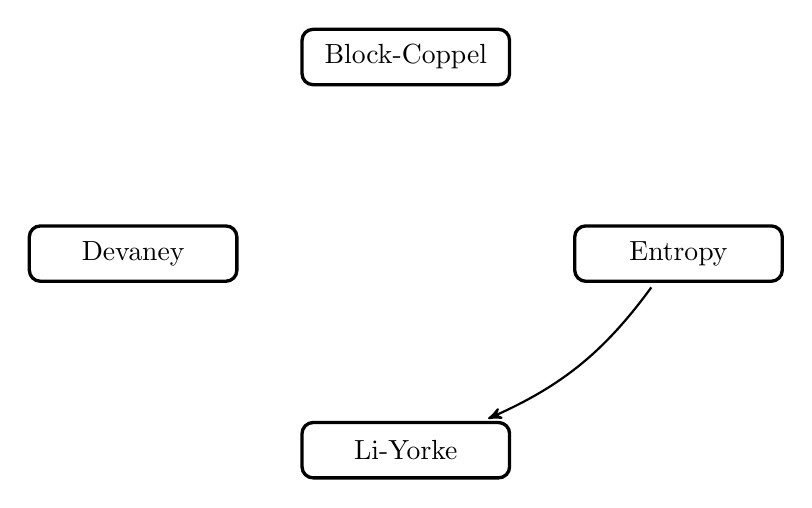
\begin{tikzpicture}[node distance=1cm, auto,]
 %nodes
    \node[] (dummy) {};
    \node[box, inner sep=5pt,below=2.0cm of dummy] (ly) {Li-Yorke};
    \node[box, inner sep=5pt,left=2.0cm of dummy] (dev) {Devaney};
    \node[box, inner sep=5pt,above=2.0cm of dummy] (bc) {Block-Coppel};
    \node[box, inner sep=5pt,right=2.0cm of dummy] (entropy) {Entropy};
 %edges
    \draw[imply] (entropy)[bend left=15] to node {} (ly); 
    %? \draw[induced] (bc) to node {} (ly); 
    %? \draw[imply] (bc) to[bend left=15] node {} (entropy); 
    %??? \draw[imply] (bc) to[bend right=15] node {} (dev); 
  \end{tikzpicture}
  \label{fig:chaos-metric}
  \caption{
    Relations between definitions for a compact metric space.
    An absence of an arrow means that the particular implication is not necessarily true.
    For instance, Devaney's chaos does not imply Block-Copple's chaos.
  }
\end{figure}

A system with posivite topological entropy is chaotic in Li-Yorke's sense.
\begin{theorem}
  \citep{blanchard}
  If $(X,F)$ has positive topological entropy, then it is chaotic in Li-Yorke's sense.
  \label{thm:entropy-liyorke}
\end{theorem}
As we have already seen in the compact interval case that the converse of the last theorem is not true in general.
For the same reason, LY implies neither Block-Coppel's nor Devaney's chaos.

Even if $F$ is semi-conjugate to $\sigma$, we only have $h(F) \leq h(\sigma)$.
$h(\sigma)$ is positive, but we can't conclude that $h(F)$ is positive.

\citet{aulbach} has shown that neither Li-Yorke's nor Block-Coppel's definition implies Devaney's definition.
\begin{theorem}
  \citep{aulbach} 
  The adding machine is chaotic in Li-Yorke's sense \textbf{and} in Block-Coppel's sense.
  However, the system is not chaotic in Devaney's sense.
  \begin{proof}
    (Adding machine example)
  \end{proof}
\end{theorem}

The following example is a system that is chaotic in Wiggins's sense but not in Li-Yorke's sense.
\begin{example}
  \citep{blanchard}
  Sturmian System.
  Chaos in Wiggins's sense is not a sufficient condition for chaos in Li-Yorke's sense.  
\end{example}
Obviously, this does not mean that Devaney's definition is not a sufficient condition for Li-Yorke's definition.
Is there a system that is topologically transitive and has dense periodic points but not Li-Yorke chaotic?

In summary,

\bibliographystyle{../../bibliography/pjgsm}
\bibliography{../../bibliography/thesis}

\printindex
\end{document}

